\subsection{Iterative Optimization Algorithm}
One of the drawbacks of our approach to event trigger and argument prediction was that the models were independent. As a result, any errors made in trigger prediction will cascade and affect the argument identification phase. For instance, if an event trigger is not predicted, we are going to miss all the arguments predictions for the trigger as well. At the same time, any incorrect event triggers predicted may result in lots of event-argument pairs being predicted that do not exist. Even after we used NomLex to find nominalizations, our classifier missed predicting some of the triggers. But, if we knew that there were entities that were children of the word in the dependency graph, then it gives more evidence that the word is an event trigger. At the same time if there are words that we might have predicted as triggers that do not have any entities as children in the dependency tree, they are less likely to be even triggers. Hence, we hypothesized that knowledge about entities in the sentence can help in event trigger prediction as we can use more features from the dependency tree. To test this, we used the gold entities from a sentence to add more features for event trigger prediction and we found that it gave us an F1 score boost from 0.67 to 0.82. Since gold entities are not available during the test phase, we designed a separate model that predicts entities in a sentence independent of the triggers. As before, entities are sub-trees under a parse tree node and the model predicts the probability of a node to be an entity or not. We used the same dynamic programming approach for non-overlapping constraints of entities.

\begin{figure}[t]
	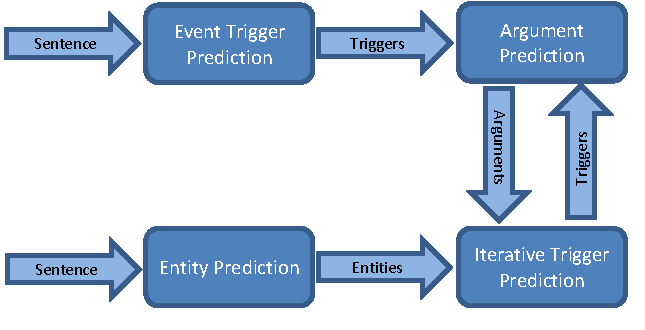
\includegraphics[width=1\columnwidth]{Images/IO}
	\caption{Stages in iterative optimization algorithm}
	\label{fig:iosteps}
\end{figure}

The different stages involved in the iterative optimization algorithm is depicted in Figure~\ref{fig:iosteps}. We use the event triggers predicted to predict its arguments. Now, we combine the set of entities predicted as arguments, with those predicted by the independent argument prediction model to create the set of all entities and is used in trigger prediction. This model predicts

$P_{IO}(T | x, A) = \prod_{e_{i}\in N_{pt}} P_{IO}(e_{i} | x, A) $, where $A$ is the set of all entities in the sentence.

Once this models predicts the event triggers, we use the same model $P_{A}(A | e,x)$ to predict arguments associtated with each event trigger that satisfy the non-overlapping constraint. Hence, $P_{IO}(A | x, e) = P_{A}(A | x, e)$. We repeat the iterative trigger and argument prediction till there is no improvement in f1 score.

TODO- Describe the featuers we used.
